\documentclass{standalone}
\usepackage{tikz}
\usepackage[T1]{fontenc} % necessary for italic font in title
\usepackage{hyperref} % for referencing
\usepackage{xcolor} % own color definitions
\usepackage{listings} % code snippets
\usepackage[normalem]{ulem} % strikethrough text
\usepackage[mathscr]{eucal} % tensor euler script
\usepackage{amsmath}
\usepackage{tabularx}
\usepackage{commath}
\usepackage{graphicx}
\usepackage[caption = false]{subfig}
\usepackage{amssymb}
\usetikzlibrary{patterns}
\usetikzlibrary{decorations.pathreplacing}
\usetikzlibrary{arrows}
\usepackage{tcolorbox}
\usetikzlibrary{calc}
\definecolor{mpiblue}{HTML}{33a5c3}
\colorlet{MPIblue}{mpiblue}
\definecolor{mpibluefont}{HTML}{17a1c1}
\colorlet{MPIbluefont}{mpibluefont}
\definecolor{mpigreen}{HTML}{007675}
\colorlet{MPIgreen}{mpigreen}
\definecolor{mpired}{HTML}{78004B}
\colorlet{MPIred}{mpired}
\definecolor{mpisand}{HTML}{ece9d4}
\colorlet{MPIsand}{mpisand}
\newcommand*\circledb[1]{\tikz[baseline=(char.base)]{
            \node[shape=circle,draw,inner sep=2pt,fill = mpiblue] (char) {#1};}}
 \newcommand*\circled[1]{\tikz[baseline=(char.base)]{
            \node[shape=circle,draw,inner sep=2pt,fill = mpired!50] (char) {#1};}}    
\begin{document}

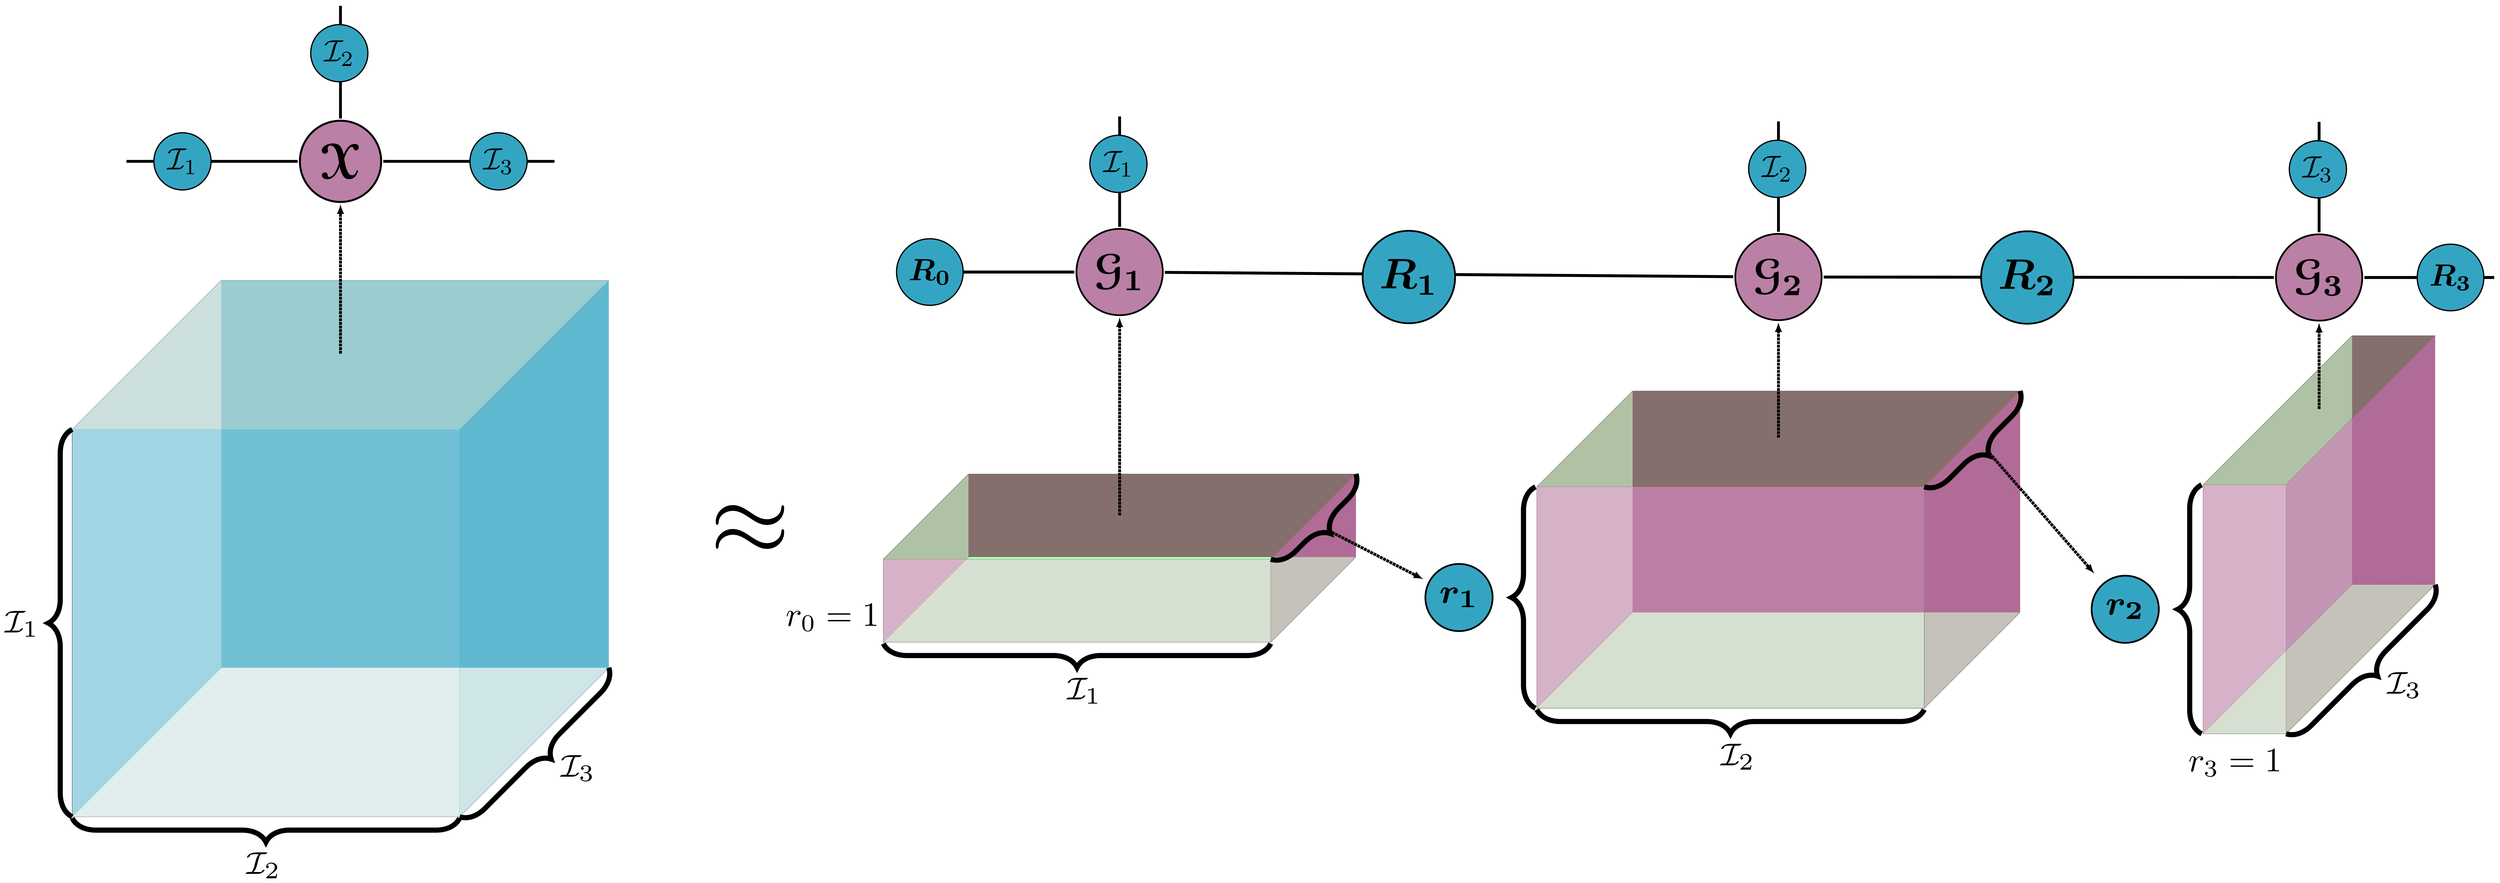
\begin{tikzpicture}
%%%%%%%%%%%%%%%%%%%%%%%%%%%%%%%%%%%%%%%%%%%%%%%%%%%%%%%%%%%%%%%%%%%%%%%%%%%%%%%%%%%%%%%%%%%%
	%% middle tt-core%%%
	\coordinate (A1) at (0em,0cm,0cm); % central top point (To pick)
	\coordinate (A2) at (1.4cm,0cm,0cm);
	\coordinate (A3) at (0em,0.8cm,0cm); % central bottom point (To pick)
	\coordinate (A4) at (0em,0cm,0.9cm);
	\coordinate (A5) at (1.4cm,0.8cm,0cm);
        \coordinate (A6) at (1.4cm,0cm,0.9cm);
        \coordinate (A7) at (0em,0.8cm,0.9cm);
        \coordinate (A8) at (1.4cm,0.8cm,0.9cm);
        
        %% Possibly draw front lines
	\draw[thick] (A3) -- (A5);
	\draw[thick] (A3) -- (A7);
	\draw[thick] (A2) -- (A6);
	\draw[thick] (A4) -- (A6); %node[below = 1cm, xshift = -30cm ] {\scalebox{15.5}{$\mathcal{I}_2$}};
	\draw[thick] (A8) -- (A5);
	\draw[thick] (A8) -- (A7);
	\draw[thick] (A8) -- (A6);
	\draw[thick] (A4) -- (A7); %node[below = 13cm,left = 0.4cm ] {\scalebox{15.5}{$r_1$}};
	\draw[thick,dashed] (A1) -- (A2) ;
 	\draw[thick,dashed] (A1) -- (A4); % node[above = 7cm, right = 6cm ] {\scalebox{15.5}{$r_2$}};
 	\draw[thick,dashed] (A1) -- (A3);
	%% Possibly draw back faces

	\fill[mpired!70] (A1) -- (A2) -- (A5) -- (A3) -- cycle; % face 6
	
 	\fill[mpired!50,opacity = 0.6] (A1) -- (A4) -- (A7) -- (A3) -- cycle; % face 3
	
	\fill[mpired!50, opacity = 0.6] (A2) -- (A5) -- (A8) -- (A6) -- cycle; % face 3
	
	\fill[mpired!30, opacity = 0.5] (A4) -- (A6) -- (A8) -- (A7) -- cycle; % face 4
	
	\fill[green!50,opacity=0.2] (A1) -- (A2) -- (A6) -- (A4) -- cycle; % f2
	
	\fill[green!90,opacity=0.2] (A3) -- (A5) -- (A8) -- (A7) -- cycle; % f5
	\node (G2) at (barycentric cs:A3=1,A5=1,A8=1,A7=1) {};
	\node (G2') [above = 12cm] at (G2) {\scalebox{12.5}{\circled{$\boldsymbol{\mathscr{G}_2}$}}};
	\node (G2'') [above = 16cm] at (G2') {};
%%%%%%%%%%%%%%%%%%%%%%%%%%%%%%%%%%%%%%%%%%%%%%%%%%%%%%%%%%%%%%%%%%%%%%%%%%%%%%%%%%%%%%%%%%%%%
         %% 1st TT-core %%
         
        \coordinate (B1) at (-2.4cm,0.2cm,0cm); % central top point (To pick)
	\coordinate (B2) at (-1cm,0.2cm,0cm);
	\coordinate (B3) at (-2.4cm,0.5cm,0cm); % central bottom point (To pick)
	\coordinate (B4) at (-2.4cm,0.2cm,0.8cm);
	\coordinate (B5) at (-1cm,0.5cm,0cm);
        \coordinate (B6) at (-1cm,0.2cm,0.8cm);
        \coordinate (B7) at (-2.4cm,0.5cm,0.8cm);
        \coordinate (B8) at (-1cm,0.5cm,0.8cm);
        
        %% Possibly draw front lines
	\draw[thick] (B3) -- (B5);
	\draw[thick] (B3) -- (B7);
	\draw[thick] (B2) -- (B6); %node[above = 3cm,right = 1cm ] {\scalebox{12.5}{$r_1$}};
	\draw[thick] (B4) -- (B6);% node[below = 1cm, xshift = -20cm ] {\scalebox{12.5}{$\mathcal{I}_1$}};
	\draw[thick] (B8) -- (B5);
	\draw[thick] (B8) -- (B7);
	\draw[thick] (B8) -- (B6);
	\draw[thick] (B4) -- (B7) node[below = 6cm, left = 0.3cm ] {\scalebox{10}{$r_0 = 1$}}; 
	\draw[thick,dashed] (B1) -- (B2) ;
 	\draw[thick,dashed] (B1) -- (B4); % 
 	\draw[thick,dashed] (B1) -- (B3);
	%% Possibly draw back faces

	\fill[mpired!70] (B1) -- (B2) -- (B5) -- (B3) -- cycle; % face 6
	
 	\fill[mpired!50,opacity = 0.6] (B1) -- (B4) -- (B7) -- (B3) -- cycle; % face 3
	
	\fill[mpired!50, opacity = 0.6] (B2) -- (B5) -- (B8) -- (B6) -- cycle; % face 3
	
	\fill[mpired!30, opacity = 0.5] (B4) -- (B6) -- (B8) -- (B7) -- cycle; % face 4
	
	\fill[green!50,opacity=0.2] (B1) -- (B2) -- (B6) -- (B4) -- cycle; % f2
	
	\fill[green!90,opacity=0.2] (B3) -- (B5) -- (B8) -- (B7) -- cycle; % f5
	\node (G1) at (barycentric cs:B3=1,B5=1,B8=1,B7=1) {};
	\node (G1') [above = 20.5cm] at (G1) {\scalebox{12.5}{\circled{$\boldsymbol{\mathscr{G}_1}$}}};
	\node (G1'') [above = 16cm] at (G1') {};
	\node (G1''') [left = 22cm] at (G1') {};
%%%%%%%%%%%%%%%%%%%%%%%%%%%%%%%%%%%%%%%%%%%%%%%%%%%%%%%%%%%%%%%%%%%%%%%%%%%%%%%%%%%%%%%%%%%%%%

         %% 3rd TT-core %%
         
        \coordinate (C1) at (2.6cm,0.1cm,0cm); % central top point (To pick)
	\coordinate (C2) at (2.9cm,0.1cm,0cm);
	\coordinate (C3) at (2.6cm,1cm,0cm); % central bottom point (To pick)
	\coordinate (C4) at (2.6cm,0.1cm,1.4cm);
	\coordinate (C5) at (2.9cm,1cm,0cm);
        \coordinate (C6) at (2.9cm,0.1cm,1.4cm);
        \coordinate (C7) at (2.6cm,1cm,1.4cm);
        \coordinate (C8) at (2.9cm,1cm,1.4cm);
        
        %% Possibly draw front lines
	\draw[thick] (C3) -- (C5);
	\draw[thick] (C3) -- (C7);
	\draw[thick] (C2) -- (C6);% node[above = 2.5cm, right = 3cm ,opacity = 4.9] {\scalebox{11.5}{$\mathcal{I}_3$}}; % 
	\draw[thick] (C4) -- (C6) node[below = 3cm, left = 0.3cm ] {\scalebox{10}{$r_3 = 1$}}; 
	\draw[thick] (C8) -- (C5);
	\draw[thick] (C8) -- (C7);
	\draw[thick] (C8) -- (C6);
	\draw[thick] (C4) -- (C7); %node[below = 15cm,left = 1cm ] {\scalebox{15.5}{$r_2$}};  
	\draw[thick,dashed] (C1) -- (C2) ;
 	\draw[thick,dashed] (C1) -- (C4) ;
 	\draw[thick,dashed] (C1) -- (C3);
	%% Possibly draw back faces

	\fill[mpired!70] (C1) -- (C2) -- (C5) -- (C3) -- cycle; % face 6
	
 	\fill[mpired!50,opacity = 0.6] (C1) -- (C4) -- (C7) -- (C3) -- cycle; % face 3
	
	\fill[mpired!50, opacity = 0.6] (C2) -- (C5) -- (C8) -- (C6) -- cycle; % face 3
	
	\fill[mpired!30, opacity = 0.5] (C4) -- (C6) -- (C8) -- (C7) -- cycle; % face 4
	
	\fill[green!50,opacity=0.2] (C1) -- (C2) -- (C6) -- (C4) -- cycle; % f2
	
	\fill[green!90,opacity=0.2] (C3) -- (C5) -- (C8) -- (C7) -- cycle; % f5
	\node (G3) at (barycentric cs:C3=1,C5=1,C8=1,C7=1) {};
	\node (G3') [above = 9cm] at (G3) {\scalebox{12.5}{\circled{$\boldsymbol{\mathscr{G}_3}$}}};
	\node (G3'') [above = 16cm] at (G3') {};
	\node (G3''') [right = 18cm] at (G3') {};
%%%%%%%%%%%%%%%%%%%%%%%%%%%%%%%%%%%%%%%%%%%%%%%%%%%%%%%%%%%%%%%%%%%%%%%%%%%%%%%%%%%%%%%%%%%%%%
         %%Main tensor %%
          %% 1st TT-core %%
         
        \coordinate (x1) at (-5.1cm,-0.2cm,0cm); % central top point (To pick)
	\coordinate (x2) at (-3.7cm,-0.2cm,0cm);
	\coordinate (x3) at (-5.1cm,1.2cm,0cm); % central bottom point (To pick)
	\coordinate (x4) at (-5.1cm,-0.2cm,1.4cm);
	\coordinate (x5) at (-3.7cm,1.2cm,0cm);
        \coordinate (x6) at (-3.7cm,-0.2cm,1.4cm);
        \coordinate (x7) at (-5.1cm,1.2cm,1.4cm);
        \coordinate (x8) at (-3.7cm,1.2cm,1.4cm);
        
        %% Possibly draw front lines
	\draw[thick] (x3) -- (x5);
	\draw[thick] (x3) -- (x7);
	\draw[thick] (x2) -- (x6); 
	\draw[thick] (x4) -- (x6);
	\draw[thick] (x8) -- (x5);
	\draw[thick] (x8) -- (x7);
	\draw[thick] (x8) -- (x6);
	\draw[thick] (x4) -- (x7); 
	\draw[thick,dashed] (x1) -- (x2) ;
 	\draw[thick,dashed] (x1) -- (x4); % 
 	\draw[thick,dashed] (x1) -- (x3);
	%% Possibly draw back faces

	\fill[mpiblue!90] (x1) -- (x2) -- (x5) -- (x3) -- cycle; % face 6
	
 	\fill[mpiblue!70,opacity = 0.6] (x1) -- (x4) -- (x7) -- (x3) -- cycle; % face 3
	
	\fill[mpiblue!70, opacity = 0.6] (x2) -- (x5) -- (x8) -- (x6) -- cycle; % face 3
	
	\fill[mpiblue!50, opacity = 0.5] (x4) -- (x6) -- (x8) -- (x7) -- cycle; % face 4
	
	\fill[mpisand!50,opacity=0.5] (x1) -- (x2) -- (x6) -- (x4) -- cycle; % f2
	
	\fill[mpisand!90,opacity=0.5] (x3) -- (x5) -- (x8) -- (x7) -- cycle; % f5
	\node (X1) at (barycentric cs:x3=1,x5=1,x8=1,x7=1) {};
	\node (X1') [above = 15.5cm] at (X1) {\scalebox{14.5}{\circled{$\boldsymbol{\mathscr{X}}$}}};
	\node (X1'') [above = 16cm] at (X1') {};
	\node (X1''') [left = 22cm] at (X1') {};
	\node (X1'''') [right = 22cm] at (X1') {};
	
	\draw[-latex,line width=3mm,dotted] (X1) -- (X1') ;
	\draw[line width=3mm] (X1') -- (X1'') node [below = 5cm, left = -3cm] {\scalebox{9}{\circledb{$\mathcal{I}_2$}}};
        \draw[line width=3mm] (X1') -- (X1''') node [left = -9cm] {\scalebox{9}{\circledb{$\mathcal{I}_1$}}};
        \draw[line width=3mm] (X1') -- (X1'''') node [right = -9cm] {\scalebox{9}{\circledb{$\mathcal{I}_3$}}};
        
        \draw [line width = 15pt,decorate,decoration={brace,amplitude=70pt,mirror,raise=4pt},xshift=300pt,yshift=5pt]
 (x4) -- (x6) node[below = 5cm, left = 18cm]
{\footnotesize {\scalebox{11.5}{$\mathcal{I}_2$}}}; 
        \draw [line width = 15pt,decorate,decoration={brace,amplitude=70pt},xshift=300pt,yshift=5pt]
 (x4) -- (x7) node[below = 20cm, left = 3cm]
{\footnotesize {\scalebox{11.5}{$\mathcal{I}_1$}}};
        \draw [line width = 15pt,decorate,decoration={brace,amplitude=70pt},xshift=300pt,yshift=5pt]
 (x2) -- (x6) node[above = 5cm, right = 10cm]
{\footnotesize {\scalebox{11.5}{$\mathcal{I}_3$}}};

        \node [inner sep=0pt,below = 18cm, right = 38cm] at (X1) {\scalebox{30}{$\approx$}};
        
        %%% coordinate for TT train attached lines%%%
        \node (P1) at (barycentric cs:B2=1,B5=1,B6=1,B8=1) {};
        \node (P2) at (barycentric cs:A1=1,A4=1,A7=1,A3=1) {};
        \node (P3) at (barycentric cs:A2=1,A5=1,A8=1,A6=1) {};
        \node (P4) at (barycentric cs:C1=1,C4=1,C7=1,C3=1) {};

        %% drawing line 
        \draw[-latex,line width=3mm,dotted] (G1) -- (G1') ;
        \draw[-latex,line width=3mm,dotted] (G2) -- (G2') ;
        \draw[-latex,line width=3mm,dotted] (G3) -- (G3') ;
        \draw[line width=3mm] (G1') -- (G2') node [xshift = -38cm]{\scalebox{12.5}{\circledb{$\boldsymbol{R_1}$}}}; % circled R_1 above cores and in between dimension circles
        \draw[line width=3mm] (G2') -- (G3') node [xshift = -30cm]{\scalebox{12.5}{\circledb{$\boldsymbol{R_2}$}}}; % circled R_2 above cores and in between dimension circles
        \draw[line width=3mm] (G1') -- (G1'') node [below = 5cm, left = -3cm] {\scalebox{9}{\circledb{$\mathcal{I}_1$}}}; % circled I_1 above 1st core
        \draw[line width=3mm] (G2') -- (G2'') node [below = 5cm, left = -3cm] {\scalebox{9}{\circledb{$\mathcal{I}_2$}}}; %circled I_2 above 2nd core
        \draw[line width=3mm] (G3') -- (G3'') node [below = 5cm, left = -3cm] {\scalebox{9}{\circledb{$\mathcal{I}_3$}}}; %circled I_3 above 3rd core
        \draw[line width=3mm] (G3') -- (G3''') node [left = 1cm]{\scalebox{9}{\circledb{$\boldsymbol{R_3}$}}}; % circled R_3 
        \draw[line width=3mm] (G1') -- (G1''') node [right = -1cm]{\scalebox{9}{\circledb{$\boldsymbol{R_0}$}}}; % circled R_0
       
        \draw [line width = 15pt,decorate,decoration={brace,amplitude=70pt},xshift=300cm,yshift=5cm]
        (B5) -- (B8) node (k1) [black,midway,xshift=1.2cm, yshift = -1.25cm]  {}; % curly braces for r_1 at 1st core 
	\draw [line width = 15pt,decorate,decoration={brace,amplitude=70pt,mirror,raise=4pt},xshift=300pt,yshift=5pt]
	(A7) -- (A4) node (k2) [black,midway,xshift=-8cm] % curly braces for r_1 at 2nd core
	{\footnotesize \scalebox{12.5}{\circledb{$\boldsymbol{r_1}$}}}; % circled small r_1
	\draw [line width = 15pt,decorate,decoration={brace,amplitude=70pt},xshift=300cm,yshift=5cm]
	(A5) -- (A8) node (k3) [black,midway,xshift=1.2cm, yshift = -0.8cm]  {};
	\draw [line width = 15pt,decorate,decoration={brace,amplitude=70pt,mirror,raise=4pt},xshift=300cm,yshift=5cm]
	(C7) -- (C4) node (k4) [black,midway,xshift=-8cm] 
	{\footnotesize \scalebox{12.5}{\circledb{$\boldsymbol{r_2}$}}}; % circled small r_2
	\draw[-latex,line width=3mm,dotted] (k1) -- (k2) ;
	\draw[-latex,line width=3mm,dotted] (k3) -- (k4) ;
	\draw [line width = 15pt,decorate,decoration={brace,amplitude=70pt,mirror,raise=4pt},xshift=300pt,yshift=5pt]
	(B4) -- (B6) node[below = 5cm, left = 17cm]
	{\footnotesize {\scalebox{11.5}{$\mathcal{I}_1$}}};   % below first core
	\draw [line width = 15pt,decorate,decoration={brace,amplitude=70pt,mirror,raise=4pt},xshift=300pt,yshift=5pt]
	(A4) -- (A6) node[below = 5cm, left = 17cm]
	{\footnotesize {\scalebox{11.5}{$\mathcal{I}_2$}}}; % below 2nd core
	\draw [line width = 15pt,decorate,decoration={brace,amplitude=70pt},xshift=300pt,yshift=5pt]
	(C2) -- (C6) node[above = 5cm, right = 10cm ,opacity = 4.9]
	{\footnotesize {\scalebox{11.5}{$\mathcal{I}_3$}}};       % below 3rd core
        
\end{tikzpicture}
\end{document} 